\begin{center}

  \begin{tabular}{rp{6cm}lp{12cm}}%{rl}

  % after \\: \hline or \cline{col1-col2} \cline{col3-col4} ...

  论文地址:& \href{https://arxiv.org/abs/1611.07308}{https://arxiv.org/abs/1611.07308} \\

  源码:& \href{https://github.com/tkipf/gae}{gae} \\

%  slides:& \href{http://yunshengb.com/wp-content/uploads/2017/03/nips_2018_r2l_workshop_talk.pdf}{{\footnotesize Convolutional Set Matching for Graph Similarity}}\\

  关键词:& \textbf{Variational auto encoders} \\

  写于:& \date{2020-10-16}

  \end{tabular}

\end{center}

该论文\cite{kipf2016variational}利用VAE(Variational auto-encoder\cite{kingma2014autoencoding})来学习无向图的隐表示,并可以从隐表示解码出原来的图。

\begin{figure}[h]
	\centering
	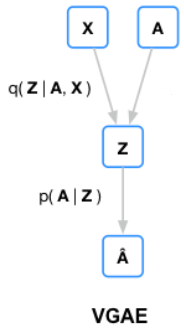
\includegraphics[width=.13\textwidth]{pics/VGAE.PNG}
	\caption{VGAE}
	\label{fig:vgae}
\end{figure}

\paragraph{VGAE思路}模型的思路如图Fig.\ref{fig:vgae}所示。其中$X \in \mathbb{R}^{N \times D}, A \in \mathbb{R}^{N \times N}$分别是无向图$G$的结点特征矩阵、邻接矩阵,$Z \in \mathbb{R}^{N \times F}$是$G$的隐表示,$\hat{A} \in \mathbb{R}^{N \times N}$是通过隐表示解码出的图的邻接矩阵,相当于根据隐表示重建后的图的邻接矩阵。整个模型可以看作一个VAE模型,分为编码和解码两个阶段。从$(X, A)$到$Z$通过GCN来完成,从$Z$到$\hat{A}$则是通过隐表示间的内积再通过激活函数得到边的概率。

\paragraph{方法解决的问题/优势}
\begin{itemize}
	\item 提出使用VAE模型对图进行编码和解码
	\item 在对图进行编/解码的过程中,隐表示$Z$可以视作结点表征

\end{itemize}

\paragraph{方法的局限性/未来方向}
\begin{itemize}
	\item 个人感觉编码过程略粗糙,不精细
	\item 扩展性不好
\end{itemize}

在看这篇论文之前,我以为这篇论文的重点是图的重建,但是文中更多地体现的是获得隐表示,将隐表示用于下游任务。那么,\tbc{red}{能否学习一个图编码器,能够很好地对图进行压缩,重建时又可能准确呢?}



